\section{Bit manipulation}
\begin{itemize}
  \item Bit masking: set, clear, toggle and test group of bites
\end{itemize}
In this section I will explian some bit manipulation operations. As it's common in most programing tasks and to avoid difficult cases: we will foucus on positive values for integer types.

Just to clarify the terms: \emph{bit} is a single binary digit, it can have only two values either 0 or 1. A \emph{byte} is a group of bits that conforms the unit of the computer architecture. Technically, a byte can have any size in bits. However, in modern computers this is always 8. That is why sometimes they call a byte an \emph{octet}. For the following code samples you can assume the following constant to be in scope.

\begin{minted}{cpp}
const size_t BITS_PER_BYTE = 8U;
\end{minted}

Let me introduce, in Listing~\ref{lst:binHelpers}; two helper function to debug and visulize such variables. The first one: \mintinline{cpp}{bitSize} returns the size in bits of the variable and the second one: \mintinline{cpp}{bitStr} returns a string with the binary representation of a variable.

{\centering
\begin{minipage}{\linewidth}
  \begin{listing}[H]
  \inputminted[
  xleftmargin=1.5cm,  %without this option line number goes wrong
  %frame=lines,
  framesep=0.5cm,
  baselinestretch=1.2,
  fontsize=\footnotesize,
  linenos,
  firstline=76, %If you omit this two fields, the whole file is pulled
  lastline=86
  ]{cpp}{src/bitOperations.cpp}
  \caption{Helper functions to debug bit manipulations}
  \label{lst:binHelpers}
  \end{listing}
\end{minipage}
\par
}

Another important feature in C++ is that we can use binary (since standar C++14) and heaxadecimal literals:
\begin{minted}{cpp}
unsigned char aChar = 0b101010;
int anInt = 0xFF00FF08;
cout << "binary representation of aChar: " << binStr(aChar) << endl;
cout << "binary representation of anInt: " << binStr(anInt) << endl;
\end{minted}
The above code will print:
\begin{verbatim}
binary representation of aChar: 00101010
binary representation of anInt: 11111111000000001111111100001000
\end{verbatim} 

\subsection{Bit's operations}

The operations that work at bits level are the following:
\begin{itemize}
\item Shift to the left by $n$ bits. Performed with the operator \mintinline{cpp}{<<}.
\item Shift to the right by $n$ bits. Performed with the operator \mintinline{cpp}{>>}.

These binary operations take an integer value (in the left hand side) and an unsigned integer value (in the right hand side) and return the result of an integer value of the same size of the left operand created by shifting the bits of the left operand by the number of bits represented by the right operand.
The bits shifted out are descarted and in order to fill the spaces created by the shift, zeros are inserted.
Because of this, shifting to any side by the exact size in bits of the left operand is the same as setting the result to 0.
However, a quick warning note: Shifting to any side by a number greater than the size (in bits) of the left operand or by a negative number it is not defined. See~\cite{INT34Cpp} for a more detailed explanation.

The code snippet in Listing~\ref{lst:bitShifting} shows a valid C++ sample of these operations:

{\centering
\begin{minipage}{\linewidth}
  \begin{listing}[H]
  \inputminted[
  xleftmargin=1.5cm,  %without this option line number goes wrong
  %frame=lines,
  framesep=0.5cm,
  baselinestretch=1.2,
  fontsize=\footnotesize,
  linenos,
  firstline=36, %If you omit this two fields, the whole file is pulled
  lastline=47
  ]{cpp}{src/bitOperations.cpp}
  \caption{Sample of bit shiting}
  \label{lst:bitShifting}
  \end{listing}
\end{minipage}
\par
}

Produces the following output:

\begin{verbatim}
a: 00101010 = 42
b: 01010000 = 80
c: 00000101 = 5
d: 00000000 = 0
e: 00000000 = 0
\end{verbatim} 

Another important thing to notice is that, \emph{as long as the shift leaves significant digits} (or else we \emph{underflow}); shifting values to the right is equivalent to divide by $2^n$ where $n$ is the number of bits shifted.
Similarly, shifting values to the left, \emph{as long as we do not discard a significant bit} (or else we \emph{overflow}); is equivalent to multiply by $2^n$, where $n$ is the number of bits shifted.
Note also that unsigned types cannot underflow.

In the above sample $2^3 = 8$. Therfore: $e = 42 / 8 = 5$ (remember it's an integer division).
And $d = 42 \cdot 8 = 336$, but it resulted in an overflow, since the maximun value for an $8$ bit variable is $2^8 = 256$.

\item Bitwise \emph{AND} between two values of the same size. Performed with the operator \mintinline{cpp}{&}. Yes, it is the same as the \emph{dereference} operator. The distinctions is made due the former being a binary operator and the dereference one being a unary operator.
\item Bitwise \emph{OR} between two values of the same size. Performed with the operator \mintinline{cpp}{|}
\item Bitwise \emph{XOR} between two values of the same size. Also known as \emph{exclusive or}. Performed with the operator \mintinline{cpp}{^}

These operators are the expected equivalent to the ones defined in first order logic.
However, they operate bitwise; that is why they are different than the logical ones that are represented by double ampersand or double pipe.

\item Bitwise unary \emph{NOT}. Performed with the operator \mintinline{cpp}{~}
\end{itemize}

Listing~\ref{lst:bitwiseOp} present a sample usage of the bitwise logical operations:

{\centering
\begin{minipage}{\linewidth}
  \begin{listing}[H]
  \inputminted[
  xleftmargin=1.5cm,  %without this option line number goes wrong
  %frame=lines,
  framesep=0.5cm,
  baselinestretch=1.2,
  fontsize=\footnotesize,
  linenos,
  firstline=50, %If you omit this two fields, the whole file is pulled
  lastline=71
  ]{cpp}{src/bitOperations.cpp}
  \caption{Bitwise operations sample}
  \label{lst:bitwiseOp}
  \end{listing}
\end{minipage}
\par
}

And produces the following result:

\begin{verbatim}
c = a & b
a: 10101101
b: 11100110
c: 10100100
d = a | b
a: 10101101
b: 11100110
d: 11101111
e = a ^ b
a: 10101101
b: 11100110
e: 01001011
f = ~a
a: 10101101
f: 01010010
\end{verbatim}

\subsection{Bit manipulations}

In order to do bit manipulations, we need to be able to refer to a specific bit.
The bits on a variable are refered by a position.
The first position, is the rightmost bit; its refered as $0$ positions continue to increment by one to the left until the last bit.
Look at the Figure~\ref{fig:bitPos}
Therefore, in an $8$ bit size variable positions are in $\{ 0, 1, \ldots, 6, 7 \}$ and in a $32$ bit variable are in $\{ 0, 1, \ldots, 30, 31 \}$.

\begin{figure}[htb]
  \centering
  \begin{subfigure}[b]{0.35\textwidth}
    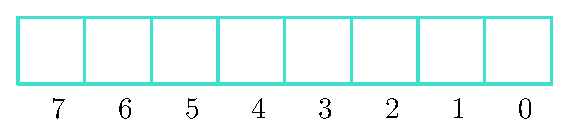
\includegraphics[width=\textwidth]{img/bitPositions}
    \caption{Bit positions for an $8$ bit variable.}
    \label{fig:bitPosa}
  \end{subfigure}
  \hspace*{1cm}
  \begin{subfigure}[b]{0.35\textwidth}
    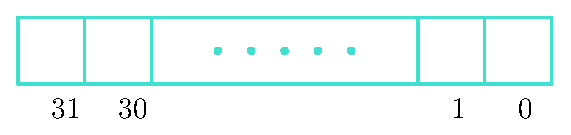
\includegraphics[width=\textwidth]{img/bitPositions2}
    \caption{Bit positions for an $32$ bit variable.}
    \label{fig:bitPosb}
  \end{subfigure}
  \caption{Positions of the bits in a variable.}
  \label{fig:bitPos}
\end{figure}

Extra note: \emph{endianism does not matter for bit manipulations}.
The languaje (in this case C++) abstract this for you.
Endianism only matters when you are reading or writing to the filesystem.
So, for the purposes of this explanation: all machines are big endian.

There are four important operations for bit manipulation:
\begin{description}
\item[Set] Put in an specific bit to the value of $1$.
\item[Clear] Put in an specific bit to the value of $0$. Also known as \emph{reset} or \emph{unset}.
\item[Toggle] Change the value of a specific bit. In other words: if the bit is $1$ set it to $0$, else set it to $1$.
\item[Query] This operation results in a boolean value. If an specif bit is $1$ return \mintinline{cpp}{true}, else return \mintinline{cpp}{false}.
\end{description}

In order to implement the bit manipulation we have to use the bit operations in combination with what is called a \emph{mask}.
A mask is another variable of the same size of the one we want to manipulate, that only contain ones in the places we want to manipulate.
Well, technically a mask could be of any size, but the explanation get easier if you imagine them of the same size.

As an example, lets construct an $8$ bit mask for manipulating the bit at position $3$.
\begin{itemize}
 \item We start with the value of $1$, in binary representation: $00000001$.
 \item Now, we shift to the left by $n$ bits. Where $n$ is the desired position.
 \item In other words to construct the mask we could do: \mintinline{cpp}{1 << 3}.
 \item The mask is: $00001000$
\end{itemize}

Now that we have the mask, it becomes obvious that we can use it to operate it with the variable to manipulate the bit corresponding to the mask.
For example, to set the bit at position $2$ of a variable, we make a bitwise $OR$ between the corresponding mask and the variable.
The result is a new value that has the value of $1$ at the place where the mask is pointing, and it's equall to the original variable in all the other positions.

\begin{minted}{cpp}
unsigned char a = 0b00101010;
unsigned char mask = 1 << 2; // Mask for bit at postion 2
unsigned char r = a | mask;
cout << "a: " << binStr(a) << endl;
cout << "m: " << binStr(mask) << endl;
cout << "r: " << binStr(r) << endl;
\end{minted}
The previous code snippet will print:
\begin{verbatim}
a: 00101010
m: 00000100
r: 00101110
\end{verbatim}

The rest of the bit manipulations can be perfomed in a similar way by combining the bitwise operations and the mask.
The long code sample in Listing~\ref{lst:bitManip} shows explicitlly how to archive the bit manipulations.

{\centering
\begin{minipage}{\linewidth}
  \begin{listing}[H]
  \inputminted[
  xleftmargin=1.5cm,  %without this option line number goes wrong
  %frame=lines,
  framesep=0.5cm,
  baselinestretch=1.2,
  fontsize=\footnotesize,
  linenos,
  firstline=26, %If you omit this two fields, the whole file is pulled
  lastline=59
  ]{cpp}{src/bitManipulation.cpp}
  \caption{Bit manipulation presented in a long explicit way}
  \label{lst:bitManip}
  \end{listing}
\end{minipage}
\par
}

The output of the code in Listing~\ref{lst:bitManip} is:
\begin{verbatim}
Original value
a: 00101010
Create a mask for the bit at position 2
m: 00000100
Variable to show the reult
r: 00000000
Setting a bit: r = a | mask
a: 00101010
m: 00000100
r: 00101110
Clearing a bit: r = a & (~mask)
a: 00101010
m: 00000100
~m:11111011
r: 00101010
Toggling a bit: r = a ^ mask
a: 00101010
m: 00000100
r: 00101110
Query a bit: q = ((a & mask) != 0)
The bit is false
\end{verbatim}

Finally, the above sample in Listing~\ref{lst:bitManip}, was written in a long form that prefers clarity on explanation rather than brevity in the code.
Indeed, the most common (and compact) way to perform bit manipulation opearates does not use a temporal storage for the mask.
And operates in place: using the same vairiable as operand and output.
The Listing~\ref{lst:bitManip2} shows a sample of the most common usage.

{\centering
\begin{minipage}{\linewidth}
  \begin{listing}[H]
  \inputminted[
  xleftmargin=1.5cm,  %without this option line number goes wrong
  %frame=lines,
  framesep=0.5cm,
  baselinestretch=1.2,
  fontsize=\footnotesize,
  linenos,
  firstline=24, %If you omit this two fields, the whole file is pulled
  lastline=51
  ]{cpp}{src/bitManipulation2.cpp}
  \caption{Most common way of making bit manipulations}
  \label{lst:bitManip2}
  \end{listing}
\end{minipage}
\par
}

Which produces the following output:
\begin{verbatim}
10101011
Setting the bit at position 2
10101111
Setting the bit at position 0 (nothing happens since was already set)
10101111
Clearing the bit at position 3
10100111
Clearing the bit at position 6 (nothing happens since was already clear)
10100111
Toggling the bit at position 2
10100011
The bit at position 4 is unset
10100011
The bit at position 5 is set
10100011  
\end{verbatim}

\subsection{Manipulating groups of bits}

The general case of manipulate a group of bits is done in the same way as individual bits.
Remember, that we said that a mask contain ones in the places where we want to manipulate and zeros anywhere else.
Then, to manipulate several bits at once, we just need a more general mask.

This is particlary usefull when we operate on bigger integer types, like $32$ or $64$ bit sizes.
The usual way to construct these masks is to use hexadecimal literals.
In hexadecimal each digit represent $4$ bits.
For example, to create a mask that operates on bits $6$, $7$ and $8$ of a $32$ bit variable. 

\begin{minted}{cpp}
unsigned int mask = 0x000001c0;
cout << "m: " << binStr(mask) << endl;
\end{minted}

Will print:
\begin{verbatim}
m: 00000000000000000000000111000000
\end{verbatim}

Typically an \mintinline{cpp}{unsigned char} has $8$ bits size and an \mintinline{cpp}{unsigned int} has $32$ bits size.
Therefore, the hexadecimal representation it's particularly usefull since a literal of the form $0xXX$, where the $X$ represents an hexadecimal digit; can create a mask for an \mintinline{cpp}{unsigned char}.
And a literal in the form $0xXXXXXXXX$ can do it for an \mintinline{cpp}{unsigned int}.



\section{Analytic Geometry}
\begin{itemize}
  \item Ray, line and segment representations
  \item Ray to segment intersection
  \item Projecction
  \item Point to segment distance
  \item Belonging test on simple polygons
\end{itemize}

\section{Graphics Pipeline}
\begin{itemize}
  \item Simple: Vertex and fragment
  \item Complete, all optional stages
  \item Texture pipeline
\end{itemize}
